\documentclass{article}
\usepackage[utf8]{inputenc}
\usepackage{hyperref,ragged2e,amsmath,multicol,setspace,
fancyhdr,amsfonts,tikz,pgfplots,nccmath,enumerate,verbatim}
\usepackage[a4paper, width=216mm, height=297mm, margin=3cm]{geometry}
\usepgfplotslibrary{polar,fillbetween}
\usepgflibrary{shapes.geometric}
\usetikzlibrary{calc,patterns,arrows}
\newcommand\mylog[1]{\mathop{{}^{#1}\mathrm{log}}}
\pgfplotsset{compat=1.15}
\pgfplotsset{my style/.append style={axis x line=middle, axis y line=
middle, xlabel={$x$}, ylabel={$y$}, axis equal }}
\usepackage{etoolbox}
\DeclareMathOperator{\sech}{sech}
\DeclareMathOperator{\csch}{csch}
\DeclareMathOperator{\arcsec}{arcsec}
\DeclareMathOperator{\arccot}{arcCot}
\DeclareMathOperator{\arccsc}{arcCsc}
\DeclareMathOperator{\arccosh}{arcCosh}
\DeclareMathOperator{\arcsinh}{arcsinh}
\DeclareMathOperator{\arctanh}{arctanh}
\DeclareMathOperator{\arcsech}{arcsech}
\DeclareMathOperator{\arccsch}{arcCsch}
\DeclareMathOperator{\arccoth}{arcCoth} 
\newcommand{\zerodisplayskips}{%
  \setlength{\abovedisplayskip}{0pt}%
  \setlength{\belowdisplayskip}{0pt}%
  \setlength{\abovedisplayshortskip}{0pt}%
  \setlength{\belowdisplayshortskip}{0pt}}
\pagestyle{fancy}
\fancyhf{}
\lhead{Halaman \thepage}
\rhead{Pembahasan Soal ETS 2021/2022 \\ (\href{https://instagram.com/ahmadzakiyudin_/}{@ahmadzakiyudin\_})}
\hypersetup{
    colorlinks=true,
    linkcolor=blue,
    filecolor=blue,      
    urlcolor=blue,
}
\setlength{\columnsep}{0.8cm}
\begin{document}
 \begin{titlepage}
    \vspace*{\fill}
    \begin{center}
      \Huge {PEMBAHASAN SOAL ETS \\ MATEMATIKA II \\ TAHUN 2021/2022}\\[0.4 cm]
      \huge {Ahmad Hisbu Zakiyudin}
    \end{center}
    \vspace*{\fill}
  \end{titlepage}
\makeatletter
\renewcommand*\env@matrix[1][*\c@MaxMatrixCols c]{%
  \hskip -\arraycolsep
  \let\@ifnextchar\new@ifnextchar
  \array{#1}}
\makeatother
\newcount\arrowcount
\newcommand\arrows[1]{
        \global\arrowcount#1
        \ifnum\arrowcount>0
                \begin{matrix}[c]
                \expandafter\nextarrow
        \fi
}

\newcommand\nextarrow[1]{
        \global\advance\arrowcount-1
        \ifx\relax#1\relax\else \xrightarrow{#1}\fi
        \ifnum\arrowcount=0
                \end{matrix}
        \else
                \\
                \expandafter\nextarrow
        \fi
}
\newpage
\setstretch{1.15}
\section*{SOAL KELAS 10-16}
\begin{enumerate}
	\item Dapatkan turunan $f^{-1}$ dari fungsi 
	\begin{align*}
	f(x) = 8x^7+2x^3+3x+7
	\end{align*}
	\item Hitung integral berikut:
	\begin{align*}
	\int \dfrac{dx}{\sqrt{9x^2-16}}, \left(x>\frac{4}{3}\right)
	\end{align*}
	\item Hitung integral berikut:
	\begin{align*}
	\int \dfrac{2x^2-9x-9}{x^3-9x}\, dx
	\end{align*}
	\item Hitunglah integral berikut:
	\begin{align*}
	\int_0^{\pi/3} \dfrac{\sec^2 x}{1-\tan x}\, dx
	\end{align*}
	\item Dapatkan volume benda padat yang terjadi bila daerah yang dibatasi oleh $y=\sqrt{x},y=x^2$ diputar terhadap garis $y=1$.\\
	\textbf{Penyelesaian:}\\
	\textbf{Metode Cakram}\\
	Perhatikan sketsa grafik berikut (benda putarnya gambar sendiri hehe :D)
	\begin{center}
		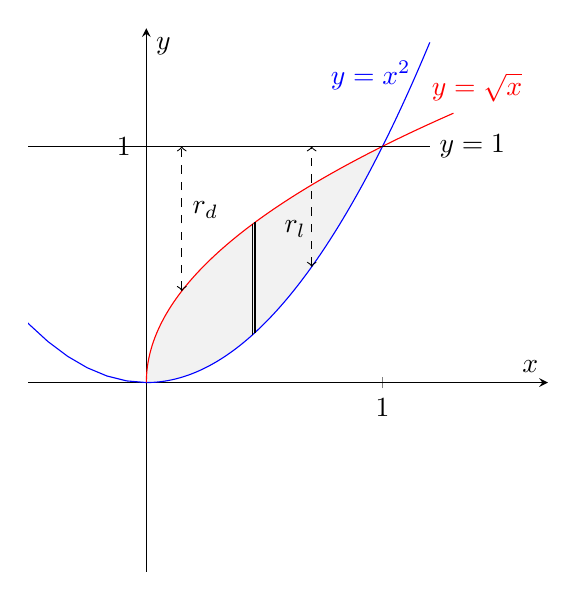
\begin{tikzpicture}
\begin{axis}[
x =3 cm, y=3 cm,
 axis lines=middle,
  xmin=-0.5,xmax=1.7,ymin=-0.8,ymax=1.5,
  xtick distance=1,
  ytick distance=1,
  xlabel=$x$,
  ylabel=$y$]
\addplot [blue,domain=0:1, samples=1000, name path=B] {x^2};
\addplot [blue,domain=1:1.2, samples=1000] {x^2};
\addplot [red,domain=0:1, samples=1000, name path=A] {sqrt(x)};
\addplot [red,domain=1:1.3] {sqrt(x)};
\addplot [blue,domain=-2:0] {x^2};
\addplot[gray,opacity=0.1] fill between[of=B and A];
\draw[dashed,<->] (0.15,0.3873) -- (0.15,1);
\draw[dashed,<->] (0.7,0.49) -- (0.7,1);
\draw (0.25,0.73) node{$r_d$};
\draw (0.63,0.65) node{$r_l$};
\draw[red] (1.4,1.25) node{$y=\sqrt{x}$};
\draw[blue] (0.95,1.3) node{$y=x^2$};
\draw (-2,1) -- (1.2,1) node [right] {$y=1$};
\draw (0.45,0.2025) -- (0.45,0.6708);
\draw (0.46,0.67823) -- (0.46,0.2116);
\end{axis}
\end{tikzpicture}
		\end{center}
		Tinjau bahwa jari-jari dalamnya adalah $r_d=1-y=1-\sqrt{x}$ dan jari-jari luar adalah $r_l=1-y=1-x^2$ serta batasnya adalah dari $x=0$ hingga $x=1$, diperoleh
		\begin{align*}
		V=\pi\int_a^b r_l^2-r_d^2 \, dx &= \pi \int_0^1 (1-x^2)^2-(1-\sqrt{x})^2\, dx\\
		&= \pi \int_0^1 1-2x^2+x^4-(1-2\sqrt{x}+x)\, dx\\
		&= \pi\left[\dfrac{x^5}{5}-\dfrac{2x^3}{3}-\dfrac{x^2}{2}+\dfrac{4x\sqrt{x}}{3}\right]^1_0\\
		&= \pi \left[\dfrac{1}{5}-\dfrac{2}{3}-\dfrac{1}{2}+\dfrac{4}{3}\right]\\
		&= \dfrac{11\pi}{30}
		\end{align*}
\end{enumerate}
\section*{SOAL KELAS 26-32}
\begin{enumerate}
	\item Hitung integral berikut:
	\begin{align*}
	\int \dfrac{\sinh \sqrt{5x}}{\sqrt{5x}}\, dx
	\end{align*}
	\textbf{Penyelesaian:}\\
	Ingat bahwa $\displaystyle \int \sinh x \, dx = \cosh x +C$. Selanjutnya misalkan $u=\sqrt{5x}$ sehingga $du = \dfrac{5}{2\sqrt{5x}}\, dx$, diperoleh 
	\begin{align*}
	\int \sinh \sqrt{5x}\, dx &= \int \sinh \
	\end{align*}
	\item Dapatkan $\dfrac{dy}{dx}$ dari 
	\begin{align*}
	y= \dfrac{x^3\sqrt[4]{5x^2+12}}{(1+x^2)^4}
	\end{align*}
	\item Hitung integral berikut:
	\begin{align*}
	\int \sin 2x\cos^2 x\, dx
	\end{align*}
	\item Hitunglah integral berikut:
	\begin{align*}
	\int_0^{+\infty} \dfrac{dx}{\sqrt{x}(x+4)}
	\end{align*}
	\item Dapatkan volume benda padat yang terjadi bila daerah yang dibatasi oleh $y=x,y=\sqrt{4-x^2},x=0$ diputar terhadap sumbu $x$.
\end{enumerate}
\section*{SOAL KELAS 34-40}
\begin{enumerate}
	\item Dapatkan $x$ dari persamaan 
	\begin{align*}
	\ln \dfrac{1}{x}+\ln 9x^4=\ln 3x
	\end{align*}
	\textbf{Penyelesaian:}\\
	Ingat bahwa $\ln a+\ln b=\ln ab$ dan $\ln a-\ln b=\ln \frac{a}{b}$ sehingga 
	\begin{align*}
	\ln \frac{1}{x}+\ln 9x^4 &= \ln 3x\\
	\ln \frac{9x^4}{x}-\ln 3x &= 0\\
	\ln \frac{9x^3}{3x} &= 0\\
	\ln 3x^2 &= 0
	\intertext{Ingat jika $y=\ln x$, maka $e^y=x$ sehingga}
	e^0 &= 3x^2
	\intertext{Karena persamaannya berlaku untuk $x>0$, diperoleh}
	x &= \dfrac{1}{\sqrt{3}}
	\end{align*}
	\item Hitung integral berikut:
	\begin{align*}
	\int x^3 3^{x^4}\, dx
	\end{align*}
	\textbf{Penyelesaian:}\\
	Misalkan $x^4=u$ sehingga $4x^3\, dx = du$ dan diperoleh 
	\begin{align*}
	\int x^3 3^{x^4} \, dx &= \int \frac{1}{4} 3^u \, du
	\intertext{Ingat bahwa $\displaystyle \int a^x \, dx = \frac{a^x}{\ln a} +C$ sehingga}
	\int x^3 3^{x^4} \, dx &= \frac{1}{4} \times \frac{3^u}{\ln 3} +C\\
	&= \frac{3^{x^4}}{4\ln 3} + C
	\end{align*}
	\item Hitung integral berikut: 
	\begin{align*}
	\int \dfrac{x^5+2x+1}{x^3-x}\, dx
	\end{align*}
	\textbf{Penyelesaian:}\\
	Perhatikan bahwa 
	\begin{align*}
	\dfrac{x^5+2x+1}{x^3-x} &= \dfrac{x^5+\color{red}(-x^3+x^3-x+x)\color{black}+2x+1}{x^3-x} \\
	&= \dfrac{x^5-x^3+x^3-x+3x+1}{x^3-x}\\
	&= \dfrac{x^2(x^3-x)}{x^3-x}+\dfrac{x^3-x}{x^3-x}+\dfrac{3x+1}{x^3-x}\\
	&= x^2+1 +\dfrac{3x+1}{x^3-x}
	\end{align*}
	Selanjutnya tinjau dekomposisi pecahan dari $\dfrac{3x+1}{x^3-x}$, yaitu 
	\begin{align*}
	\dfrac{3x+1}{x^3-x} = \dfrac{3x+1}{x(x-1)(x+1)} &= \dfrac{A}{x} + \dfrac{B}{x-1} + \dfrac{C}{x+1}\\
	&= \dfrac{A(x-1)+Bx}{x(x-1)} +\dfrac{C}{x+1}\\
	&= \dfrac{(A+B)x-A}{x(x-1)} +\dfrac{C}{x+1}\\
	&= \dfrac{((A+B)x-A)(x+1)+C(x(x-1))}{x(x-1)(x+1)}\\
	&= \dfrac{(A+B)x^2+(A+B)x-Ax-A+Cx^2-Cx}{x(x-1)(x+1)}\\
	&= \dfrac{(A+B+C)x^2+(B-C)x-A}{x(x-1)(x+1)}
	\end{align*}
	Diperoleh $A=-1, B=2, C=-1$ sehingga 
	\begin{align*}
	\int \dfrac{x^5+2x+1}{x^3-x}\, dx &= \int x^2+1 -\dfrac{1}{x}+\dfrac{2}{x-1}-\dfrac{1}{x+1} \, dx\\
	&= \dfrac{x^3}{3} + x -\ln x +2\ln |x-1| -\ln |x+1| +C 
	\end{align*}
	\item Hitunglah integral berikut 
	\begin{align*}
	\int_{-3/2}^0 \dfrac{x+2}{\sqrt{2x+3}}\, dx
	\end{align*}
	\textbf{Penyelesaian:}\\
	Misalkan $2x+3=u$ sehingga $2\, dx=du$. Untuk $x=-\dfrac{3}{2}$, maka $u=0$, dan untuk $x=0$, maka $u=3$. Diperoleh pula $x=\dfrac{u-3}{2}$ sehingga $x+2=\dfrac{u+1}{2}$. Jadi diperoleh 
	\begin{align*}
	\int_{-3/2}^0 \dfrac{x+2}{\sqrt{2x+3}}\, dx &= \int_0^3 \dfrac{u+1}{4\sqrt{u}} \, du\\
	&= \lim_{a\rightarrow 0^+} \dfrac{1}{4}\int_a^3 \sqrt{u} + u^{-\frac{1}{2}} \, du\\
	&= \lim_{a\rightarrow 0^+} \dfrac{1}{4}\left[\dfrac{2u\sqrt{u}}{3}+2\sqrt{u}\right]^3_a\\
	&= \lim_{a\rightarrow 0^+} \dfrac{1}{4}\left[2\sqrt{3}+2\sqrt{3} - \dfrac{2a\sqrt{a}}{3}-2\sqrt{a}\right] = \sqrt{3}
	\end{align*}
	\item Dapatkan volume benda padat yang terjadi bila daerah yang dibatasi oleh $y=(x-2)^2,x+y=4$ diputar pada $x=4$.\\
	\textbf{Penyelesaian:}\\
	Tinjau bahwa $y=4-x$ sehingga titik potongnya adalah 
	\begin{align*}
	4-x &= x^2-4x+4\\
	x^2-3x &= 0\\
	x(x-3) &= 0
	\end{align*}
	Untuk $x=0$, maka $y=4$, dan untuk $x=3$, maka $y=1$. Diperoleh titik potongnya adalah $(0,4)$ dan $(3,1)$. Berikut grafiknya
	\begin{center}
		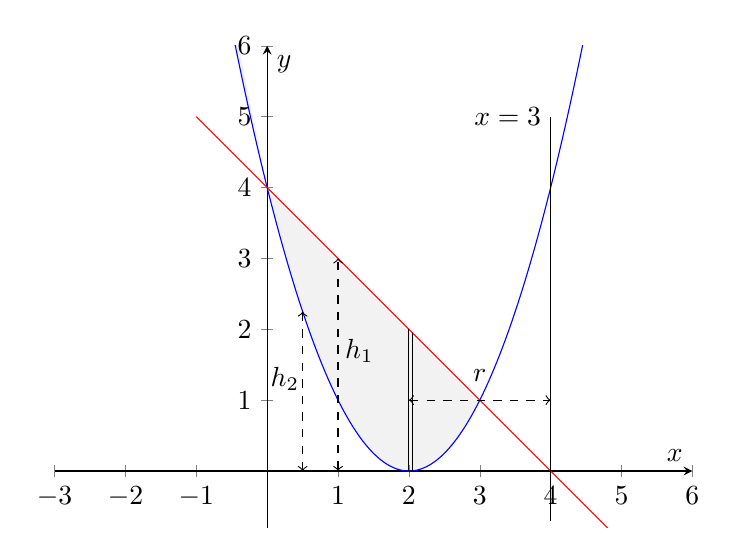
\begin{tikzpicture}
\begin{axis}[
x =.9 cm, y=.9 cm,
 axis lines=middle,
  xmin=-3,xmax=6,ymin=-0.8,ymax=6,
  xtick distance=1,
  ytick distance=1,
  xlabel=$x$,
  ylabel=$y$]
\addplot [blue,domain=-1:3, samples=1000, name path=B] {(x-2)^2};
\addplot [blue,domain=3:5, samples=1000] {(x-2)^2} node [above] {$y=(x-2)^2$};
\addplot [red,domain=0:3, samples=1000, name path=A] {4-x};
\addplot [red,domain=3:5] {4-x} node [below] {$x+y=4$};
\addplot [red,domain=-1:0] {4-x};
\addplot[gray,opacity=0.1] fill between[of=B and A];
\draw[dashed,<->] (0.5,2.25) -- (0.5,0);
\draw[dashed,<->] (1,0) -- (1,3);
\draw (0.25,1.3) node{$h_2$};
\draw (1.3,1.7) node{$h_1$};
\draw (4,-0.7) -- (4,5) node [left] {$x=3$};
\draw (2,0) -- (2,2);
\draw (2.05,0.0025) -- (2.05, 1.95);
\draw[<->,dashed] (2,1) -- (4,1);
\draw (3,1.35) node {$r$};
\end{axis}
\end{tikzpicture}
		\end{center}
	Perhatikan bahwa jika kita gunakan metode cakram, maka kita perlu membagi daerah integrasi menjadi dua bagian, yaitu untuk $0\leq y\leq 1$ dan $1\leq y\leq 4$, karena batas-batas fungsinya berbeda. Oleh karena itu, digunakan metode cincin silinder supaya lebih mudah. 
	Tinjau bahwa jari-jarinya adalah $r=4-x$ dan tingginya $h=h_1-h_2=4-x-(x-2)^2=-x^2+3x$. Batasnya adalah dari $x=0$ sampai $x=3$
	\begin{align*}
	V = 2\pi \int_a^b rh \, dx &= 2\pi \int_0^3 (4-x)(-x^2+3x)\, dx \\
	&= 2\pi \int_0^3 -4x^2 +12x+x^3-3x^2\, dx\\
	&= 2\pi \int_0^3 x^3-7x^2+12x\, dx\\
	&= 2\pi \left[\dfrac{x^4}{4}-\dfrac{7x^3}{3}+6x^2\right]^3_0\\
	&= 2\pi \left[\dfrac{81}{4}-\dfrac{189}{3}+54-0\right]\\
	&= \dfrac{45\pi}{2}
	\end{align*}
	Jadi volume benda putar yang terjadi adalah $V=\dfrac{45\pi}{2}$
\end{enumerate}
\section*{SOAL KELAS 41-47}
\begin{enumerate}
	\item Dapatkan $\dfrac{dy}{dx}$ dari 
	\begin{align*}
	y = x^2\cosh^2(\sqrt{x})
	\end{align*}
	\item Hitung integral berikut:
	\begin{align*}
	\int_{\ln 3}^{\ln 8} e^{2t} \sqrt{1+e^t}\, dt
	\end{align*}
	\item Hitung integral berikut:
	\begin{align*}
	\int \sin^{\frac{1}{3}} t\cos^3 t\, dt
	\end{align*}
	\item Dapatkan limit berikut:
	\begin{align*}
	\lim_{x\rightarrow \infty} \left(\dfrac{x-1}{x+2}\right)^x
	\end{align*}
	\item Sketsa daerah yang dibatasi oleh $y=x,y=\dfrac{1}{x},x=2,y=0$ dan dapatkan luasnya.
\end{enumerate}
\section*{SOAL KELAS 56-63}
\begin{enumerate}
	\item Dapatkan penyelesaian dari persamaan 
	\begin{align*}
	\ln (e^{-x}-1) = x
	\end{align*}
	\textbf{Penyelesaian:}\\
	Ingat bahwa jika $y=\ln x$, maka $x=e^y$ sehingga
	\begin{align*}
	\ln (e^{-x}-1) &= x\\
	e^{-x}-1 &= e^x\\
	1-e^x &= e^{2x}
	\intertext{Misalkan $e^x=u$, diperoleh}
	u^2+u-1 &= 0 \\
	u &= \dfrac{-1\pm \sqrt{1-(4)(1)(-1)}}{2(1)}\\
	&= \dfrac{-1\pm \sqrt{5}}{2}
	\intertext{Karena $e^x>0$, akibatnya}
	e^x &= \dfrac{-1+\sqrt{5}}{2}\\
	x=\ln e^x&= \ln \left(\dfrac{-1+\sqrt{5}}{2}\right)
	\end{align*}
	\item Dapatkan $\dfrac{dy}{dx}$ dari 
	\begin{align*}
	y= \tan^{-1} (xe^{3x})
	\end{align*}
	\textbf{Penyelesaian:}\\
	Ingat bahwa jika $y=\tan^{-1}(x)$, maka $\dfrac{dy}{dx} = \dfrac{1}{1+x^2}$. Selanjutnya, misalkan $p=xe^{3x}$, dengan aturan perkalian diperoleh 
	\begin{align*}
	\dfrac{dp}{dx} = 1(e^{3x}) + x(3e^{3x}) = e^{3x}+3xe^{3x}
	\end{align*}
	Dengan aturan rantai, didapatkan 
	\begin{align*}
	\dfrac{dy}{dx} &= \dfrac{dy}{dp}\dfrac{dp}{dx}\\
	&= \dfrac{1}{1+p^2}\times \left(e^{3x}+3xe^{3x}\right)\\
	&= \dfrac{e^{3x}+3xe^{3x}}{1+(xe^{3x})^2}
	\end{align*}
	\item Hitung integral berikut:
	\begin{align*}
	\int \dfrac{dx}{5+5\sin x}
	\end{align*}
	\textbf{Penyelesaian:}\\
	Misalkan $u=\tan \left(\frac{x}{2}\right)$ sehingga $2\tan^{-1}u = x$ dan $\dfrac{2}{1+u^2}\, du = dx$.\\
	Dari sini, didapatkan $\sin \left(\frac{x}{2}\right) = \dfrac{u}{\sqrt{1+u^2}}, \cos \left(\frac{x}{2}\right) = \dfrac{1}{\sqrt{1+u^2}}$ sehingga 
	$$\sin x = 2\sin\left(\frac{x}{2}\right)\cos \left(\frac{x}{2}\right) = \dfrac{2u}{1+u^2} $$
	Selanjutnya, diperoleh 
	\begin{align*}
	\int \dfrac{dx}{5+5\sin x} &= \dfrac{1}{5}\int \dfrac{dx}{1+\sin x}\\
	&= \dfrac{1}{5} \int \dfrac{1}{1+\frac{2u}{1+u^2}}\dfrac{2}{1+u^2}\, du\\
	&= \dfrac{1}{5} \int \dfrac{2}{1+u^2+2u}\, du\\
	&= \dfrac{2}{5} \int (u+1)^{-2} \, du\\
	&= -\dfrac{2}{5(u+1)} + C\\
	&= -\dfrac{2}{5\left(\tan \left(\frac{x}{2}\right) +1\right)} +C
	\end{align*}
	\item Hitung integral berikut:
	\begin{align*}
	\int_{\pi/3}^{\pi/2} \dfrac{\sin x}{\sqrt{1-2\cos x}}\, dx
	\end{align*}
	\textbf{Penyelesaian:}\\
	Misalkan $1-2\cos x=u$ sehingga $2\sin x\, dx = du$ dengan batas atas $u=1-2\cos \frac{\pi}{2} = 1$ dan batas bawah $u=1-2\cos \frac{\pi}{3} = 0$, diperoleh 
	\begin{align*}
	\int_{\pi/3}^{\pi/2} \dfrac{\sin x}{\sqrt{1-2\cos x}}\, dx &= \int_0^1 \dfrac{1}{2\sqrt{u}} \, du\\
	&= \lim_{a\rightarrow 0^+} \int_a^1 \dfrac{u^{-1/2}}{2}\, du\\
	&= \lim_{a\rightarrow 0^+} \dfrac{1}{2}\times (2u^{1/2})\bigg|^1_a\\
	&= \lim_{a\rightarrow 0^+} 1- \sqrt{a} = 1
	\end{align*}
	\item Dapatkan volume benda padat yang diperoleh bila daerah yang dibatasi oleh $y=\sqrt{x+6}, y=0, x=0$ diputar pada garis $x=3$\\
	\textbf{Penyelesaian:}\\
	\textbf{Metode Cakram}\\
	Perhatikan sketsa grafik berikut (benda putarnya gambar sendiri hehe :D) 
	\begin{center}
		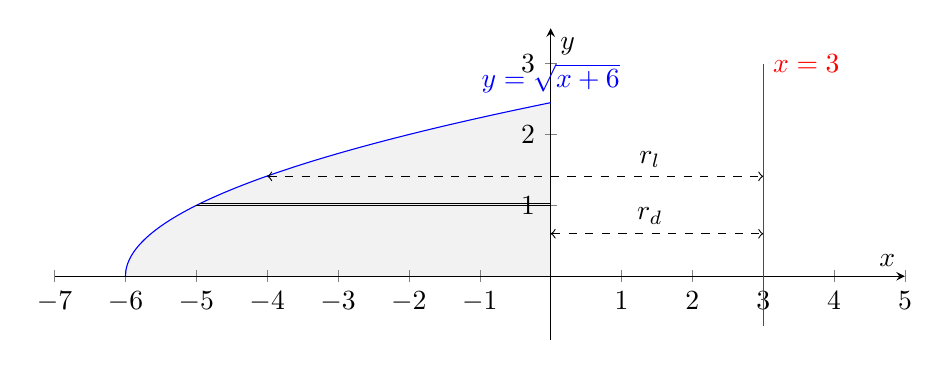
\begin{tikzpicture}
\begin{axis}[
x =.9 cm, y=.9 cm,
 axis lines=middle,
  xmin=-7,xmax=5,ymin=-0.9,ymax=3.5,
  xtick distance=1,
  ytick distance=1,
  xlabel=$x$,
  ylabel=$y$]
\addplot [blue,domain=-6:0, samples=1000, name path=B] {sqrt(x+6)} node [above] {$y=\sqrt{x+6}$};
\addplot [domain=-6:0, name path=A] {0};
\addplot[gray,opacity=0.1] fill between[of=B and A];
\draw[red] (3,-0.7) -- (3,3) node [right] {$x=3$};
\draw (-5,1) -- (0,1);
\draw (-4.95,1.025) -- (0,1.025);
\draw[<->,dashed] (-4,1.41) -- (3,1.41);
\draw (1.4,1.65) node {$r_l$};
\draw[dashed,<->] (0,0.6) -- (3,0.6);
\draw (1.4,0.85) node {$r_d$};
\end{axis}
\end{tikzpicture}
		\end{center}
	Perhatikan bahwa $x=y^2-6,y\geq 0$. \\Jari-jari dalamnya adalah $r_d=3$ dan jari-jari luar adalah $r_l=3-x=3-(y^2-6)=9-y^2$.\\
	Perhatikan bahwa batasnya adalah dari $y=0$ hingga $y=\sqrt{6}$, maka 
	\begin{align*}
	V =\pi \int_a^b r_l^2-r_d^2\, dy &= \pi\int_0^{\sqrt{6}} \left(9-y^2\right)^2-\left(3\right)^2\, dy\\
	&= \pi \int_0^{\sqrt{6}} 81-18y^2+y^4-9\, dy\\
	&= \pi\int_0^{\sqrt{6}} y^4-18y^2+72\, dy\\
	&= \pi\left[\dfrac{y^5}{5}-6y^3+72y\right]^{\sqrt{6}}_0\\
	&= \pi \left[-\dfrac{36\sqrt{6}}{5}-36\sqrt{6}+72\sqrt{6}\right] \\
	&= \dfrac{216\sqrt{6}}{5}\pi
	\end{align*}
	\textbf{Metode Cincin Silinder}\\
	Berikut adalah sketsa grafiknya, dalam hal ini $r=3-x$ sedangkan tinggnya $h=\sqrt{x+6}$
	\begin{center}
		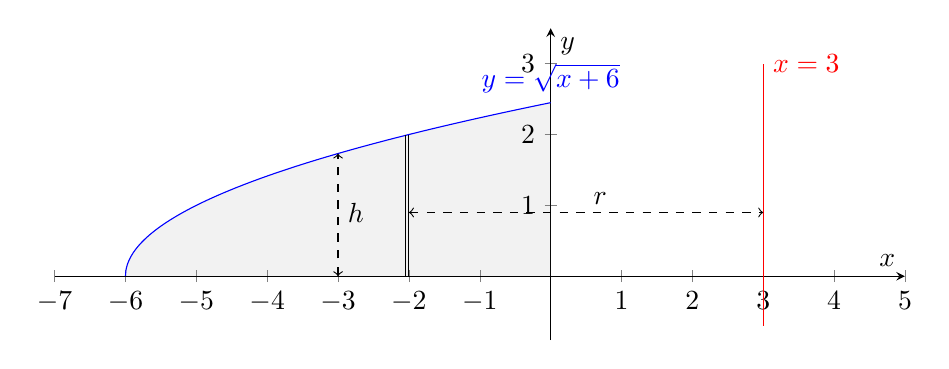
\begin{tikzpicture}
\begin{axis}[
x =.9 cm, y=.9 cm,
 axis lines=middle,
  xmin=-7,xmax=5,ymin=-0.9,ymax=3.5,
  xtick distance=1,
  ytick distance=1,
  xlabel=$x$,
  ylabel=$y$]
\addplot [blue,domain=-6:0, samples=1000, name path=B] {sqrt(x+6)} node [above] {$y=\sqrt{x+6}$};
\addplot [domain=-6:0, name path=A] {0};
\addplot[gray,opacity=0.1] fill between[of=B and A];
\draw[red] (3,-0.7) -- (3,3) node [right] {$x=3$};
\draw (-2,0) -- (-2,2);
\draw (-2.05,1.987) -- (-2.05,0);
\draw[<->,dashed] (-2,0.9) -- (3,0.9);
\draw (0.7,1.1) node {$r$};
\draw[dashed,<->] (-3,0) -- (-3,1.732);
\draw (-2.75,0.9) node {$h$};
\end{axis}
\end{tikzpicture}
		\end{center}
		Perhatikan bahwa batasnya adalah dari $x=-6$ hingga $x=0$, diperoleh 
		\begin{align*}
		V = 2\pi \int_a^b rh\, dx &= 2\pi \int_{-6}^0 (3-x)\sqrt{x+6}\, dx
		\end{align*}
		Misalkan $x+6=u$ sehingga $x=u-6$ dan $du=dx$. Untuk $x=-6$, maka $u=0$, dan untuk $x=0$, maka $u=6$, diperoleh
		\begin{align*}
		V &= 2\pi \int_0^6 (3-(u-6))\sqrt{u}\, du\\
		&= 2\pi\int_0^6 9\sqrt{u} - u\sqrt{u}\, du\\
		&= 2\pi \left[\dfrac{9(2u\sqrt{u})}{3}+\dfrac{2u^2\sqrt{u}}{5}\right]^6_0\\
		&= 2\pi \left[6(6)\sqrt{6}-\dfrac{2(6)^2\sqrt{6}}{5}\right]\\
		&= \dfrac{216\sqrt{6}}{5}\pi
		\end{align*}
		Jadi volume benda putar yang terjadi adalah $V=\dfrac{216}{5}\pi$
\end{enumerate}
\end{document}
